

\chapter{Android Boot Sequence}
\label{android_boot}
\paragraph*{•}

\hspace{8mm} 

\noindent At the core of Android is the Linux Kernel managing all the underlying hardware. Hence boot process is
similar to what we find in a Linux machine. However, the devices which run Android are highly
integrated devices, called SoCs, which have a wide range of devices which we dont find in
a normal linux desktop system or a laptop. Much of these devices come with proprietary drivers.
The bootloader usually used for ARM based SoCs, is called Uboot. However, for Intel Atom SoC
based on the Cherrytrail family uses a proprietary bootloader, called Kernelflinger.

Once Kernel is started, it does the driver initialization and call the first userspace program,
called init. From here, what init loads is making the difference as what we see Android as it is.

The diagram below shows the boot flow in Android:


\begin{figure}[h]
  \centering
    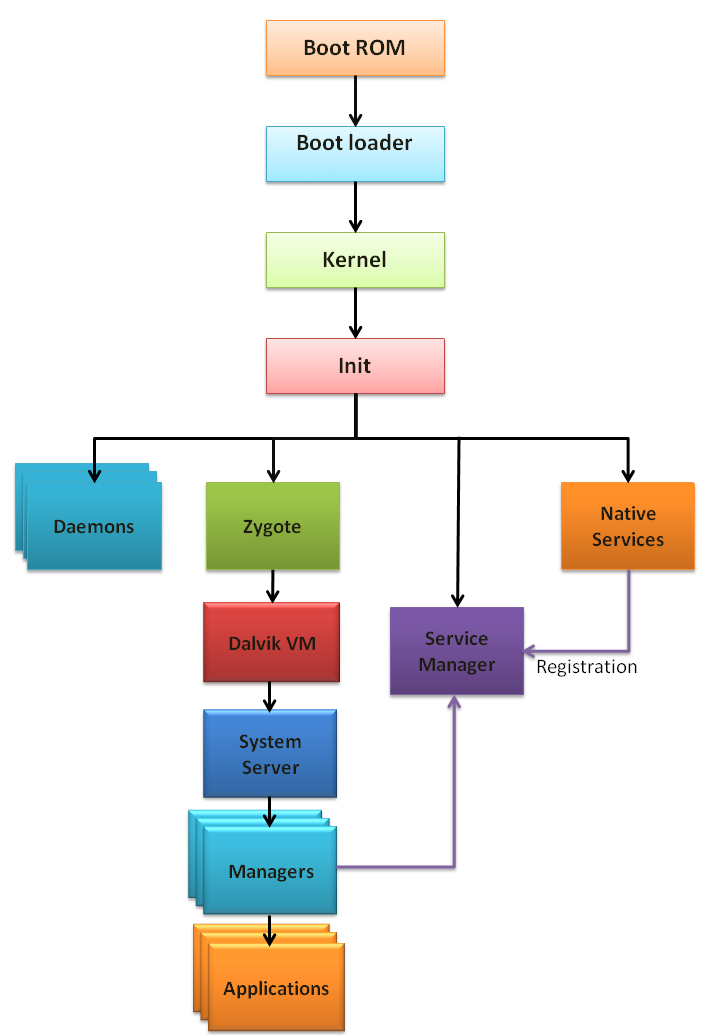
\includegraphics[scale=0.7]{android_boot.png}
    \caption{Android Boot Process}
    \label{fig:android_boot}
\end{figure}

\clearpage
\section{Bootloader}

Up on power up, the SoC firmware boots from a ROM area typically located internally,
different from the system's eMMC card. This is what we loosely call BIOS, for legacy
reasons. This code determines the boot media and loads the boot loader from the media.
The boot loader can be used to initialize the DRAM and load another level of loader
or directly the Linux kernel. On Cherrytrail Platform, the bootloader is called Kernelflinger.
It then loads the Linux Kernel with the required parameters hardcoded in the boot image.

\section{Kernel}

Linux kernel is the heart of the Android responsible for the process creation, inter process communication, device drivers, file system management etc. Android applies a custom patch on the main stream kernel to support certain features like Wake locks etc needed for operation of the Android.

The kernel is loaded as a compressed imaege. Up on loading, it decompresses itself,
does the driver initializations, mounts the root file system (typically passed 
as kernel command line arguments) and starts the first application in user space.


\section{Android}

Android typically operates wholly on the user space. The android applications are executed over a Virtual Machine called the Dalvik. The following section explains the internals in detail.

\subsection{init and init.rc}

The first user space application executed on booting the kernel is the init
executable located in the root folder. The process parses a start up script
called the \textit{init.rc} script. This is written in a language designed
for android used to start all the necessary processes, daemons and services
for a proper operation of android. It offers various types of execution timings
such as early-init, on-boot, on-post-fs etc. A detailed explanation of the
scripting model is available on Android documentation site.

\subsection{Demons and Services}

The init process creates various daemons and processes like rild, vold,
mediaserver, adb, etc each responsible for its own functionality.
Descriptions of these processes are not in the scope of this post.
Rather we will discuss more about \textit{Zygote} process.

\subsection{Service Manager}

The service manager process manages all the services running in the system.
Every service created registers itself with this process and this information
is used for future references by other processes/applications.

\subsection{Zygote}

Zygote is one of the first init process created on boot. The term ``zygote`` is based the biological ''initial cell formed
that divides to produce offsprings``. Similarly zygote in android initializes the Dalivik VM and
forks to create multiple instances to support each android process. It facilitates using a shared code
across the VM instances resulting in a low memory foot print and short load time, ideal for an embedded system.

Zygote apart from installing a listener on the server socket, also preloads classes and
resources to be used later in the Android applications. Once done, the system server is started.

%nbegin{figure}[h]
%  \centering
%  \begin{subfigure}[b]{1\textwidth}
%    \centering
%    \includegraphics[scale=0.4]{digraph_simple.png}
%    \caption{Relation digraph of the simplified system}
%    \label{fig:digraph_simple}
%  \end{subfigure}
  
%  \begin{subfigure}[b]{1\textwidth}
%    \centering
%    \includegraphics[scale=0.4]{digraph_virtual.png}
%    \caption{Representation of the digraph with virtual nodes}
%    \label{fig:digraph_virtual}
%  \end{subfigure}
  
%\end{figure}

